\setcounter{section}{0}
\section{Hình thành kiến thức mới}

\subsection{Mở đầu}
Thời xa xưa, hiện tượng Mặt Trời hoặc Mặt Trăng đột ngột bị che khuất hoàn toàn bởi một tác nhân vô hình trong một khoảng thời gian luôn gây ra cho con người sự kinh hoàng, bởi con người thời đó lo sợ sự biến mất vĩnh viễn của Mặt Trời hoặc Mặt Trăng. Ngoài ra, sự thay đổi của mực nước sông, biển đã được ông cha ta vận dụng nhằm che giấu các bãi cọc cắm dưới lòng sông để đánh thắng quân thù. Những hiện tượng đó có thể được giải thích như thế nào?
\subsection{Hình thành kiến thức mới}

Hiện tượng nhật thực, nguyệt thực là hiện tượng che khuất lẫn nhau do Mặt Trăng chuyển động quanh Trái Đất và Trái Đất chuyển động quanh Mặt Trời.
\subsubsection{Nhật thực}
Hiện tượng nhật thực được quan sát vào ban ngày, xảy ra trong thời gian Mặt Trăng đi qua giữa Trái Đất và Mặt Trời. Lúc đó, người quan sát từ Trái Đất sẽ thấy Mặt Trăng che khuất hoàn toàn hay một phần Mặt Trời.
\begin{center}
	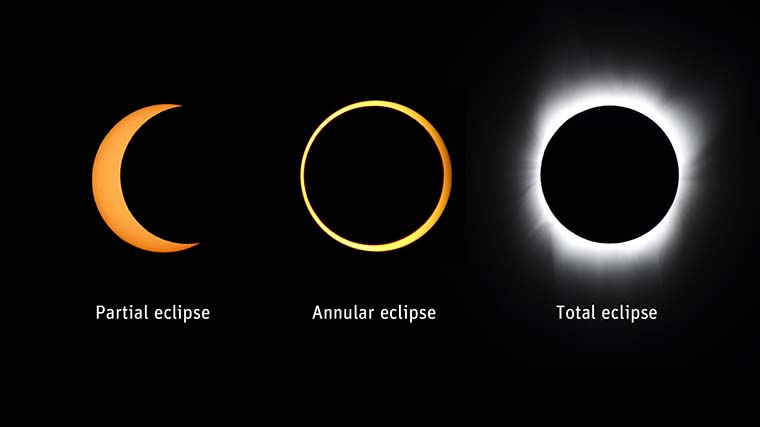
\includegraphics[width=0.6\linewidth]{../figs/G10-035-1}
\end{center}

Quá trình diễn ra nhật thực: Đầu tiên, đĩa tối của Mặt Trăng bắt đầu tiến vào và che khuất bờ bên phải của Mặt Trời. Sau đó, đĩa tối của Mặt Trăng tiếp tục tiến dần và che khuất tâm Mặt Trời. Đến pha cực đại, nếu người quan sát ở vị trí vùng bóng tối của Mặt Trăng, thì sẽ quan sát được nhật thực trung tâm. Tùy vào vị trí của Mặt Trời, Mặt Trăng và Trái Đất mà ta có thể quan sát thấy các kiểu nhật thực khác nhau:
\begin{center}
	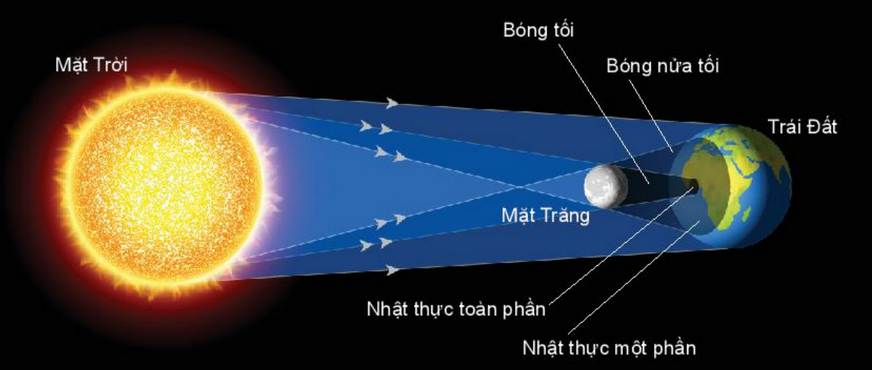
\includegraphics[width=0.6\linewidth]{../figs/G10-035-2}
\end{center}
\begin{itemize}
	\item Khi ở trong vùng bóng tối của Mặt Trăng, người quan sát sẽ thấy Mặt Trời bị đĩa tối Mặt Trăng che khuất hoàn toàn. Đây là nhật thực toàn phần.
	\item Nếu vùng bóng tối của Mặt Trăng không chạm đến Trái Đất, người quan sát sẽ thấy một vành sáng xung quanh đĩa tối của Mặt Trăng. Đây là nhật thực hình khuyên.
	\item Nhật thực một phần xảy ra khi Mặt Trời, Mặt Trăng và Trái Đất không hoàn toàn nằm trên cùng một đường thẳng, khi đó Mặt Trăng chỉ che khuất một phần của Mặt Trời.
\end{itemize}

\subsubsection{Nguyệt thực}
Vào thời kì trăng tròn, Mặt Trăng có thể chuyển động vào phần bóng tối của Trái Đất. Khi này, Mặt Trăng không còn được Mặt Trời chiếu sáng nữa và do đó, con người trên Trái Đất quan sát thấy Mặt Trăng bị che khuất vào ban đêm. Đó chính là hiện tượng nguyệt thực.
\begin{center}
	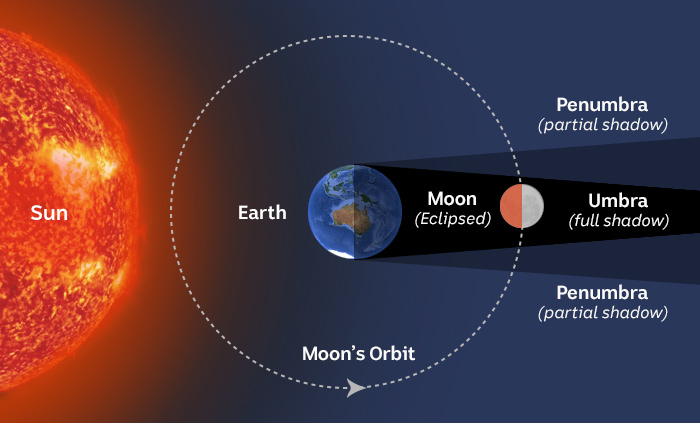
\includegraphics[width=0.6\linewidth]{../figs/G10-035-3.jpg}
\end{center}
Khác với nhật thực, hiện tượng nguyệt thực có thể được quan sát ở toàn bộ vùng tối của Trái Đất. Nguyệt thực toàn phần có thể kéo dài trong vài giờ, trong khi nhật thực toàn phần chỉ kéo dài trong vài phút.
\begin{itemize}
	\item Nguyệt thực toàn phần xảy ra khi ánh sáng chiếu trực tiếp từ Mặt Trời đến Mặt Trăng bị Trái Đất che hoàn toàn. Lúc này ánh trăng sẽ bị mờ đi và Mặt Trăng sẽ có màu đỏ hồng hoặc màu cam sẫm.
	\item Nguyệt thực một phần xảy ra khi chỉ một phần của Mặt Trăng đi vào bóng tối của Trái Đất. Lúc này ánh trăng sẽ bị mờ đi và Mặt Trăng bị khuyết đi một phần.
\end{itemize}

\subsubsection{Thủy triều}
Thủy triều là hiện tượng nước biển, nước sông, ... lên xuống theo quy luật xác định. Chu kì của thủy triều đúng bằng khoảng thời gian giữa hai lần liên tiếp Mặt Trăng di chuyển qua vị trí đó trên bầu trời tại nơi đó

Hiện tượng mực nước dâng lên và hạ xuống thấp trong một ngày lần lượt được gọi là triều cao và triều thấp.

Nguyên nhân gây ra thủy triều là do sự khác biệt về lực hấp dẫn do Mặt Trăng và Mặt Trời tác dụng vào các phần khác nhau của lớp nước bao phủ bề mặt Trái Đất gây ra. Do Mặt Trời ở xa Trái Đất hơn nhiều so với Mặt Trăng nên thủy triều do Mặt Trời tạo ra nhỏ hơn thủy triều do Mặt Trăng tạo ra.

Vì Mặt Trăng chuyển động quanh Trái Đất và Trái Đất quay mỗi ngày một vòng quanh trục của nó nên kết quả là mỗi nơi trên mặt đất đã lần lượt có nước dâng (thủy triều lên hay "nước lớn") và nước rút (thủy triều xuống hay "nước ròng").

\begin{minipage}{0.6\textwidth}
	\begin{itemize}
		\item Vào những ngày mà Mặt Trăng, Mặt Trời và Trái Đất thẳng hàng (giao hội/ xung đối), thủy triều lên xuống mạnh hơn nên được gọi là triều cường.
		\item Ngược lại, khi hướng của Mặt Trời và Mặt Trăng so với Trái Đất vuông góc nhau (thượng huyền/ hạ huyền), thủy triều lên xuống yếu nên được gọi là triều kém.
	\end{itemize}
\end{minipage}
\begin{minipage}{0.4\textwidth}
	\begin{center}
		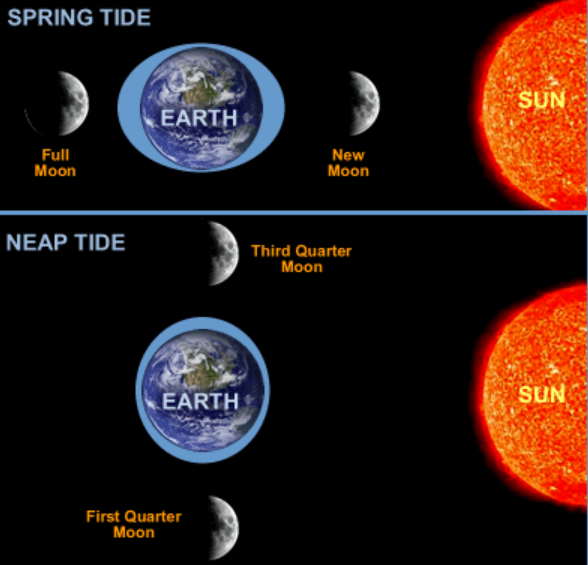
\includegraphics[scale=0.45]{../figs/G10-035-4}
	\end{center}
	
\end{minipage}
\luuy{Hiện tượng thủy triều được xét như trên có tính chất lí thuyết. Trong thực tế, chế độ thủy triều ở từng nơi diễn ra phức tạp hơn so với lí thuyết này. Một trong các nguyên nhân là do cấu tạo địa chất ở từng nơi cản trở sự lưu thông của nước.}
\subsection{Mở rộng}
\subsubsection{Hiện tượng trăng máu}
\begin{minipage}{0.6\textwidth}
	Khi xảy ra nguyệt thực toàn phần, ánh sáng duy nhất nhìn thấy được là khúc xạ qua bóng tối của Trái Đất. Ánh sáng này có màu đỏ vì cùng lý do hoàng hôn có màu đỏ, do sự tán xạ Rayleigh của các tia sáng màu có bước sóng ngắn hơn. Bởi vì màu đỏ của nó, nguyệt thực toàn phần đôi khi được gọi là mặt trăng máu.
\end{minipage}
\begin{minipage}{0.4\textwidth}
	\begin{center}
		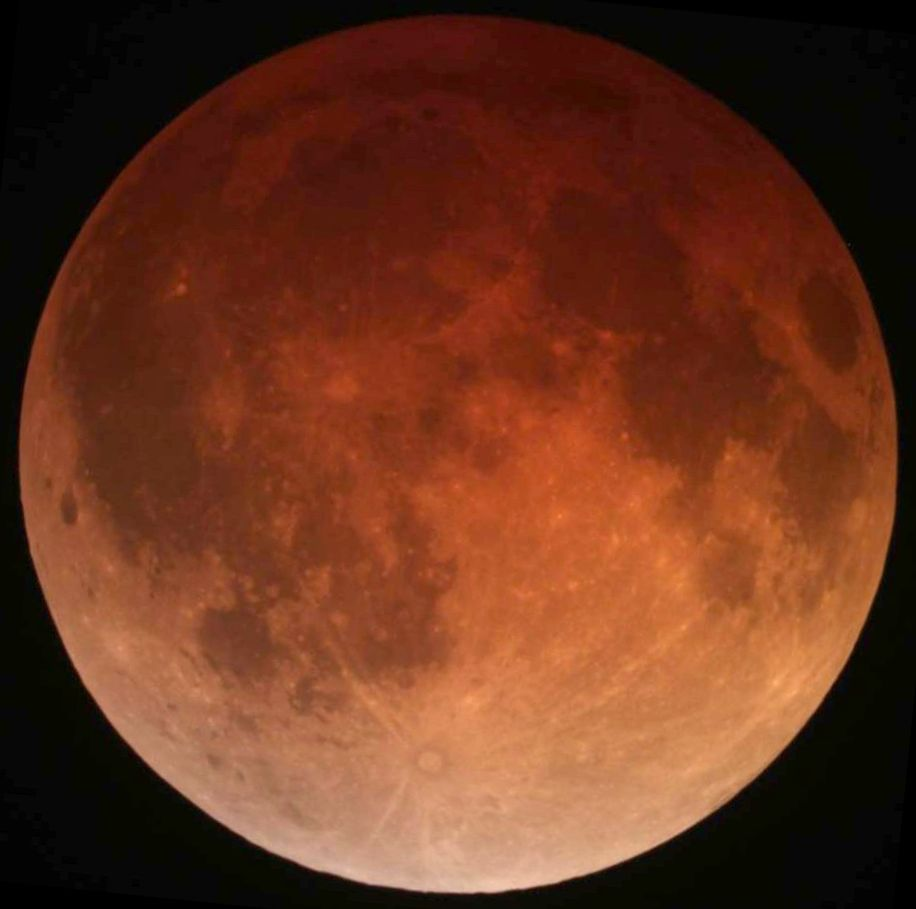
\includegraphics[width=0.5\linewidth]{../figs/G10-035-5}
	\end{center}
	
\end{minipage}

\subsubsection{Siêu trăng}
Siêu Mặt Trăng hay siêu trăng là khi Mặt Trăng vào thời kì trăng tròn hoặc trăng non trùng vào điểm cận địa, tức là điểm trên quỹ đạo của Mặt Trăng mà có khoảng cách gần nhất so với Trái Đất, làm cho kích thước biểu kiến của nó to hơn bình thường khi quan sát từ Trái Đất.
\subsubsection{Mặt Trời giả}
Mặt Trời giả hay Mặt Trời ma là một hiện tượng quang học khí quyển, gồm đốm sáng ở một hoặc cả hai bên của Mặt Trời. Hai Mặt Trời giả thường nằm ở hai bên Mặt Trời trong vòng hào quang $22^\circ$.
\begin{center}
	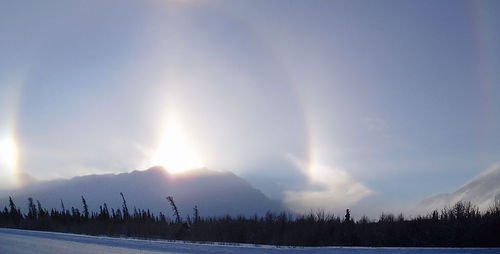
\includegraphics[width=0.6\linewidth]{../figs/G10-035-6}
\end{center}
Mặt Trời giả là một loại hào quang được tạo ra do sự khúc xạ ánh sáng mặt trời bởi các tinh thể băng trong khí quyển. Mặt Trời giả thông thường xuất hiện như một đốm màu của ánh sáng ở bên trái hoặc bên phải của Mặt Trời, vị trí khoảng $22^\circ$ ở bên trái và bên phải Mặt Trời, cùng độ cao với Mặt Trời so với đường chân trời. Chúng có thể được nhìn thấy ở bất cứ đâu trên thế giới tại bất kì thời điểm nào trong năm. Mặt Trời giả dễ thấy nhất khi ở gần đường chân trời.
\section{Mục tiêu bài học - Ví dụ minh họa}
\begin{dang}{Giải thích được hiện tượng nhật thực}
	\viduii{1}{Hãy mô tả quá trình diễn ra nhật thực.
	}
	{	\begin{center}
			\textbf{Hướng dẫn trả lời}
		\end{center}
		
		Quá trình diễn ra nhật thực: Đầu tiên, đĩa tối của Mặt Trăng bắt đầu tiến vào và che khuất bờ bên phải của Mặt Trời. Sau đó, đĩa tối của Mặt Trăng tiếp tục tiến dần và che khuất tâm Mặt Trời. Đến pha cực đại, nếu người quan sát ở vị trí vùng bóng tối của Mặt Trăng, thì sẽ quan sát được nhật thực trung tâm. Tùy vào vị trí của Mặt Trời, Mặt Trăng và Trái Đất mà ta có thể quan sát thấy các kiểu nhật thực khác nhau:
		\begin{itemize}
			\item Khi ở trong vùng bóng tối của Mặt Trăng, người quan sát sẽ thấy Mặt Trời bị đĩa tối Mặt Trăng che khuất hoàn toàn. Đây là nhật thực toàn phần.
			\item Nếu vùng bóng tối của Mặt Trăng không chạm đến Trái Đất, người quan sát sẽ thấy một vành sáng xung quanh đĩa tối của Mặt Trăng. Đây là nhật thực hình khuyên.
			\item Nhật thực một phần xảy ra khi Mặt Trời, Mặt Trăng và Trái Đất không hoàn toàn nằm trên cùng một đường thẳng, khi đó Mặt Trăng chỉ che khuất một phần của Mặt Trời.
		\end{itemize}
	}
	\viduii{2}{Việc dùng mắt để quan sát trực tiếp nhật thực có an toàn không? Giải thích và trình bày một số phương pháp để quan sát nhật thực.
	}
	{	\begin{center}
			\textbf{Hướng dẫn trả lời}
		\end{center}
		
		So với các hiện tượng thiên văn khác, việc quan sát nhật thực khá đơn giản do không cần phải dùng đến kính thiên văn. Người quan sát chỉ cần một tầm nhìn đủ lớn và bầu trời quang mây để có thể nhìn thấy Mặt Trời. 
		
		Trong quá trình diễn ra nhật thực, bức xạ từ ánh sáng Mặt Trời có thể tác động xấu tới mắt do thời gian quan sát lâu hơn bình thường. Do vậy, người xem không nên quan sát Mặt Trời bằng mắt thường trong thời điểm diễn ra nhật thực. 
		
		Người quan sát cũng không nên sử dụng các thiết bị viễn vọng như kính thiên văn, ống nhòm để quan sát trực tiếp Mặt trời bởi chúng có thể làm tăng đáng kể cường độ bức xạ tiếp xúc với mắt.
		
		Cách an toàn nhất để quan sát nhật thực đó là quan sát đĩa Mặt Trời một cách gián tiếp. Bằng cách sử dụng ống nhòm hoặc kính thiên văn với tờ bìa một lỗ nhỏ đặt trước kính và chiếu ảnh Mặt Trời lên một tờ giấy trắng.
		
		Hoặc đơn giản hơn, người xem cần chuẩn bị một chiếc kính lọc ánh sáng dành cho mắt hoặc một lớp kính lọc chuyên dụng (sun filter) nếu quan sát bằng kính thiên văn. Những chiếc kính lọc được thiết kế riêng để quan sát trực tiếp nhật thực gọi là solar glasses.
		
	}
\end{dang}
\begin{dang}{Giải thích được hiện tượng nguyệt thực}
	\viduii{1}{Hãy mô tả quá trình diễn ra nguyệt thực.
	}
	{	\begin{center}
			\textbf{Hướng dẫn trả lời}
		\end{center}
		
		Nguyệt thực là hiện tượng Mặt Trăng bị che khuất khi đi vào vùng bóng tối phía sau Trái Đất. Khi đó, vị trí của Mặt Trời, Trái Đất và Mặt Trăng nằm trên cùng một đường thẳng.
		
		Ta biết rằng cả Trái Đất và Mặt Trăng cùng chuyển động xung quanh Mặt Trời, do vậy sẽ có lúc Mặt Trăng đi vào phần bóng tối của Trái Đất, bị bóng tối của Trái Đất che khuất, khi đó xảy ra hiện tượng nguyệt thực. Nguyệt thực xảy ra trong những đêm trăng rằm, lúc ấy ta thấy Mặt Trăng bị che khuất dần, Trái Đất đã chắn hết ánh sáng của Mặt Trời nên Mặt Trăng không nhận được ánh sáng của Mặt Trời, do đó Mặt Trăng không thể phản xạ lại để chúng ta nhìn thấy đĩa sáng của nó.
		
		So với Trái Đất, đường kính của Mặt Trăng chỉ bằng một phần tư, khoảng cách từ Mặt Trăng tới Trái Đất khá gần so với khoảng cách từ Trái Đất tới Mặt Trời. Vì vậy khi xảy ra hiện tượng nguyệt thực thì toàn bộ Mặt Trăng đều nằm trong bóng tối của Trái Đất.
		
		
	}
	\viduii{2}{Hãy giải thích các loại nguyệt thực: nguyệt thực toàn phần, nguyệt thực bán phần, nguyệt thực một phần.
	}
	{	\begin{center}
			\textbf{Hướng dẫn trả lời}
		\end{center}
		
		Nguyệt thực luôn xảy ra vào dịp trăng tròn, khi Mặt Trời, Trái Đất và Mặt Trăng thẳng hàng với nhau. Trái Đất được Mặt Trời chiếu sáng luôn hắt bóng vào không gian. Khi Mặt Trăng chui hoàn toàn vào cái bóng ấy thì xảy ra pha nguyệt thực toàn phần.
		
		Khi Mặt Trăng bị che hoàn toàn, do hiện tượng khúc xạ, tán xạ của khí quyển Trái Đất nên Mặt Trăng không hoàn toàn tối đen mà có màu đỏ sẫm. Khi Mặt Trăng ở vào phần nửa tối của bóng tối Trái Đất, ta sẽ thấy nguyệt thực bán phần. Khi Mặt Trăng không hoàn toàn nằm trong vùng tối của Trái Đất, tức khi Mặt Trăng ở xa Trái Đất, vùng bóng tối chỉ chạm vào một phần của Mặt Trăng, ta có nguyệt thực một phần.
	}
\end{dang}
\begin{dang}{Giải thích được hiện tượng thủy triều}
	\viduii{2}{Giải thích tại sao khi Mặt Trời, Trái Đất và Mặt Trăng thẳng hàng sẽ xảy ra triều cường?
	}
	{	\begin{center}
			\textbf{Hướng dẫn trả lời}
		\end{center}
		
		Nguyên nhân chính của thủy triều là do lực hấp dẫn giữa Mặt Trăng với Trái Đất và giữa Trái Đất với Mặt Trời.
		
		Trong những ngày Mặt Trăng, Trái Đất và Mặt Trời thẳng hàng, lực hấp dẫn của Mặt Trời tác dụng lên Trái Đất trở nên lớn hơn. Khi đó, tại vị trí thẳng hàng, lực tác dụng lên Trái Đất sẽ là tổng hợp giữa Trái Đất - Mặt Trăng và Trái Đất - Mặt Trời, làm thủy triều lên xuống mạnh hơn, gọi là triều cường.
		
		
	}
\end{dang}
\section{Tự luận}
\begin{enumerate}[label=\bfseries Câu \arabic*:]
	\item \mkstar{2}
	
	{
		Nêu điều kiện xảy ra hiện tượng nguyệt thực và nhật thực.
	}
	
	\hideall{
		
		Nguyệt thực khi sự che khuất của Mặt trăng xảy ra, thì Mặt trời, Trái đất và Mặt trăng phải sắp thẳng hàng lúc trăng tròn. Nguyệt thực xảy ra khi Mặt trăng đi vào vùng bóng của Trái đất. Chúng có thể được nhìn thấy từ bất kì nơi nào có Mặt trăng mọc lên trước lúc bị che khuất.
		
		Nhật thực xuất hiện khi Mặt trăng đi qua phía trước Mặt trời và đổ bóng lên một phần bề mặt Trái đất. Sự che khuất hoàn toàn của Mặt trời chỉ xảy ra trong một khu vực hẹp, do cái bóng của Mặt trăng khi đổ lên Trái đất là nhỏ. Người quan sát đứng bên ngoài khu vực toàn phần này chỉ trông thấy nhật thực một phần.
	}
	
	\item \mkstar{2}
	
	
	{
		Mặt Trăng ở vị trí nào so với Trái Đất và Mặt Trời sẽ xảy ra nhật thực?
	}
	
	\hideall
	{
		Hiện tượng nhật thực xảy ra khi Mặt trăng, Mặt trời và Trái đất cùng nằm trên một mặt phẳng, thẳng hàng hoặc gần thẳng hàng với nhau. Lúc này, Mặt trăng sẽ nằm ở giữa Trái đất và Mặt trời.
	}
	\item \mkstar{3}
	
	
	{
		Hiện tượng nhật thực, nguyệt thực mỗi năm thường xảy ra như thế nào?
	}
	
	\hideall
	{
		Bất kỳ năm nào cũng sẽ có tối thiểu là bốn lần nhật, nguyệt thực: Hai lần nhật thực và hai lần là nguyệt thực. Con số này có thể nhiều hơn, tùy vào từng năm, nhưng lại không thể có 8 lần trong một năm. Đây là những hiện tượng tự nhiên của vũ trụ, đang dần được các nhà khoa học khám phá.
	}
	\item \mkstar{3}
	
	
	{
		Phân biệt nhật thực toàn phần và nhật thực hình khuyên. Nêu vai trò của Mặt Trăng trong hai hiện tượng này.
	}
	
	\hideall
	{
		\textbf{ Nhật thực toàn phần: }Xảy ra khi mặt trời bị che khuất bởi mặt trăng tạo ra các vùng tối và bóng nửa tối xuất hiện trên bề mặt trái đất. Hiện tượng nhật thực toàn phần này chỉ có thể diễn ra khi mặt trăng tiếp cận được với quỹ đạo.
		
		\textbf{Nhật thực hình khuyên:} Xảy ra khi trung tâm của đĩa mặt trời sẽ bị đĩa của mặt trăng bị che khuất. Lúc này, các phần rìa bên ngoài của Mặt Trời sẽ bị lộ ra và nhìn giống như một chiếc nhẫn. Hiện tượng nhật thực hình khuyên xảy ra khi mặt trăng ở xung quanh viễn điểm quỹ đạo.
	}
	\item \mkstar{3}
	
	
	{
		Giải thích tại sao nguyệt thực lại kéo dài hơn so với nhật thực.
	}
	
	\hideall
	{
		Trái Đất to hơn Mặt Trăng, nên bóng của Trái Đất cũng to hơn. Dẫn tới việc bóng của Trái Đất che Mặt Trăng lâu hơn.
		
	}
	\item \mkstar{2}
	
	{
		Hiện tượng thủy triều có phải là nguyên nhân chính làm cho mực nước trên các đại dương ngày càng dâng cao hay không?
	}
	
	\hideall{
		
		Hiện tượng thủy triều không phải là nguyên nhân chính làm cho mực nước trên các đại dương ngày càng dâng cao, mực nước càng dâng cao do biến đổi khí hậu làm băng tan ở hai cực.
	}
	
	\item \mkstar{2}
	
	
	{
		Vào những ngày Mặt Trăng có hình dạng như thế nào thì thủy triều lên, xuống: mạnh nhất, yếu nhất?
	}
	
	\hideall
	{
		Lúc trăng non và trăng tròn thủy triều là mạnh nhất.
	}
	\item \mkstar{2}
	
	
	{
		Giải thích tại sao khi Mặt Trời, Trái Đất và Mặt Trăng thẳng hàng sẽ xảy ra triều cường.
	}
	
	\hideall
	{
		Ngày 15, 16 âm Lịch (ngày trăng tròn): Mặt Trăng đối xứng với Mặt Trời qua Trái Đất. Tại thời điểm này, Mặt Trăng gần Trái đất hơn, lực hấp dẫn lên trục cảm ứng mạnh, từ đó tạo nên hiện tượng triều cường.
	}
	\item \mkstar{3}
	
	
	{
		Hãy mô tả diễn biến của hiện tượng nguyệt thực.
	}
	
	\hideall
	{
		Thời điểm Mặt Trăng, Trái Đất, Mặt Trời thẳng hàng nhau, ánh sáng của Mặt Trời chiếu đến Mặt Trăng bị Trái Đất chặn lại, tức là Mặt Trăng bị khuất sau bóng Trái Đất nên bị tối đen dần. Thời điểm và hiện tượng này được gọi là nguyệt thực.
		
		Do Trái Đất chỉ chắn được một phần ánh sáng Mặt Trời nên nguyệt thực chỉ có thể xảy ra khi Mặt Trăng đi qua một số vùng của bóng Trái Đất.
		
		Như vậy, nguyệt thực chỉ có thể xảy ra vào dịp trăng tròn và khi Mặt Trăng đi qua một số vùng của bóng Trái Đất.
	}
	\item \mkstar{3}
	
	
	{
		Hãy giải thích hiện tượng thủy triều.
	}
	
	\hideall
	{
		Sức hút của nhau giữa Mặt trăng và Trái đất lại có xu hướng làm cho chúng xích lại gần nhau hơn. Nhưng sức hút này sẽ được bù bằng lực quay ly tâm của Trái đất, cũng như là của Mặt trăng, quay xung quanh tâm quán tính của chúng.
		
		Tại tâm Trái đất, lực ly tâm và lực hút đến từ Mặt trăng sẽ bù nhau. Nhưng đó không phải là trường hợp ở một điểm nào đó trên mặt đất vì 2 lực này thay đổi theo chiều ngược nhau: Một điểm càng xa trọng tâm Trái đất và Mặt trăng, lực ly tâm mà nó phải chịu sẽ càng lớn, và ngược lại, sức hút của Mặt trăng sẽ giảm theo khoảng cách.
		
		Vì thế, 2 lực không bù nhau trên bề mặt của Trái đất và sự chênh lệch của chúng là nguồn gốc gây nên thủy triều: Tại điểm A, lực ly tâm không đủ để cân bằng lại với sức hút, vì vậy điểm A có xu hướng dịch chuyển về phía Mặt trăng. Ngược lại, ở điểm B lực ly tâm lớn hơn so với lực của Mặt trăng, do vậy, điểm B sẽ có xu hướng rời xa nó. Đó là lý do mà trên Trái đất có hai lần thủy triều mỗi ngày.
	}
\end{enumerate}